\section{Mapa conceptual integrador de la unidad}
La Figura~\ref{fig:mapaUnidad} vincula los cuatro temas centrales: tipos de requisitos, propiedades de calidad, proceso de requisitos y contexto del sistema. Las conexiones principales muestran qué aporta cada tema a los artefactos del PFC. Tres vínculos cruzados unen la clasificación con la verificabilidad, el contexto con la identificación de necesidades y el proceso con la revisión de calidad. Este mapa se preparó a partir del contenido del informe y puede modificarse en diagrams.net con el archivo editable \texttt{figuras/mapa\_conceptual.drawio} \cite{iso29148,pohl2025,swebok2024}.
\begin{figure*}[!t]
\centering
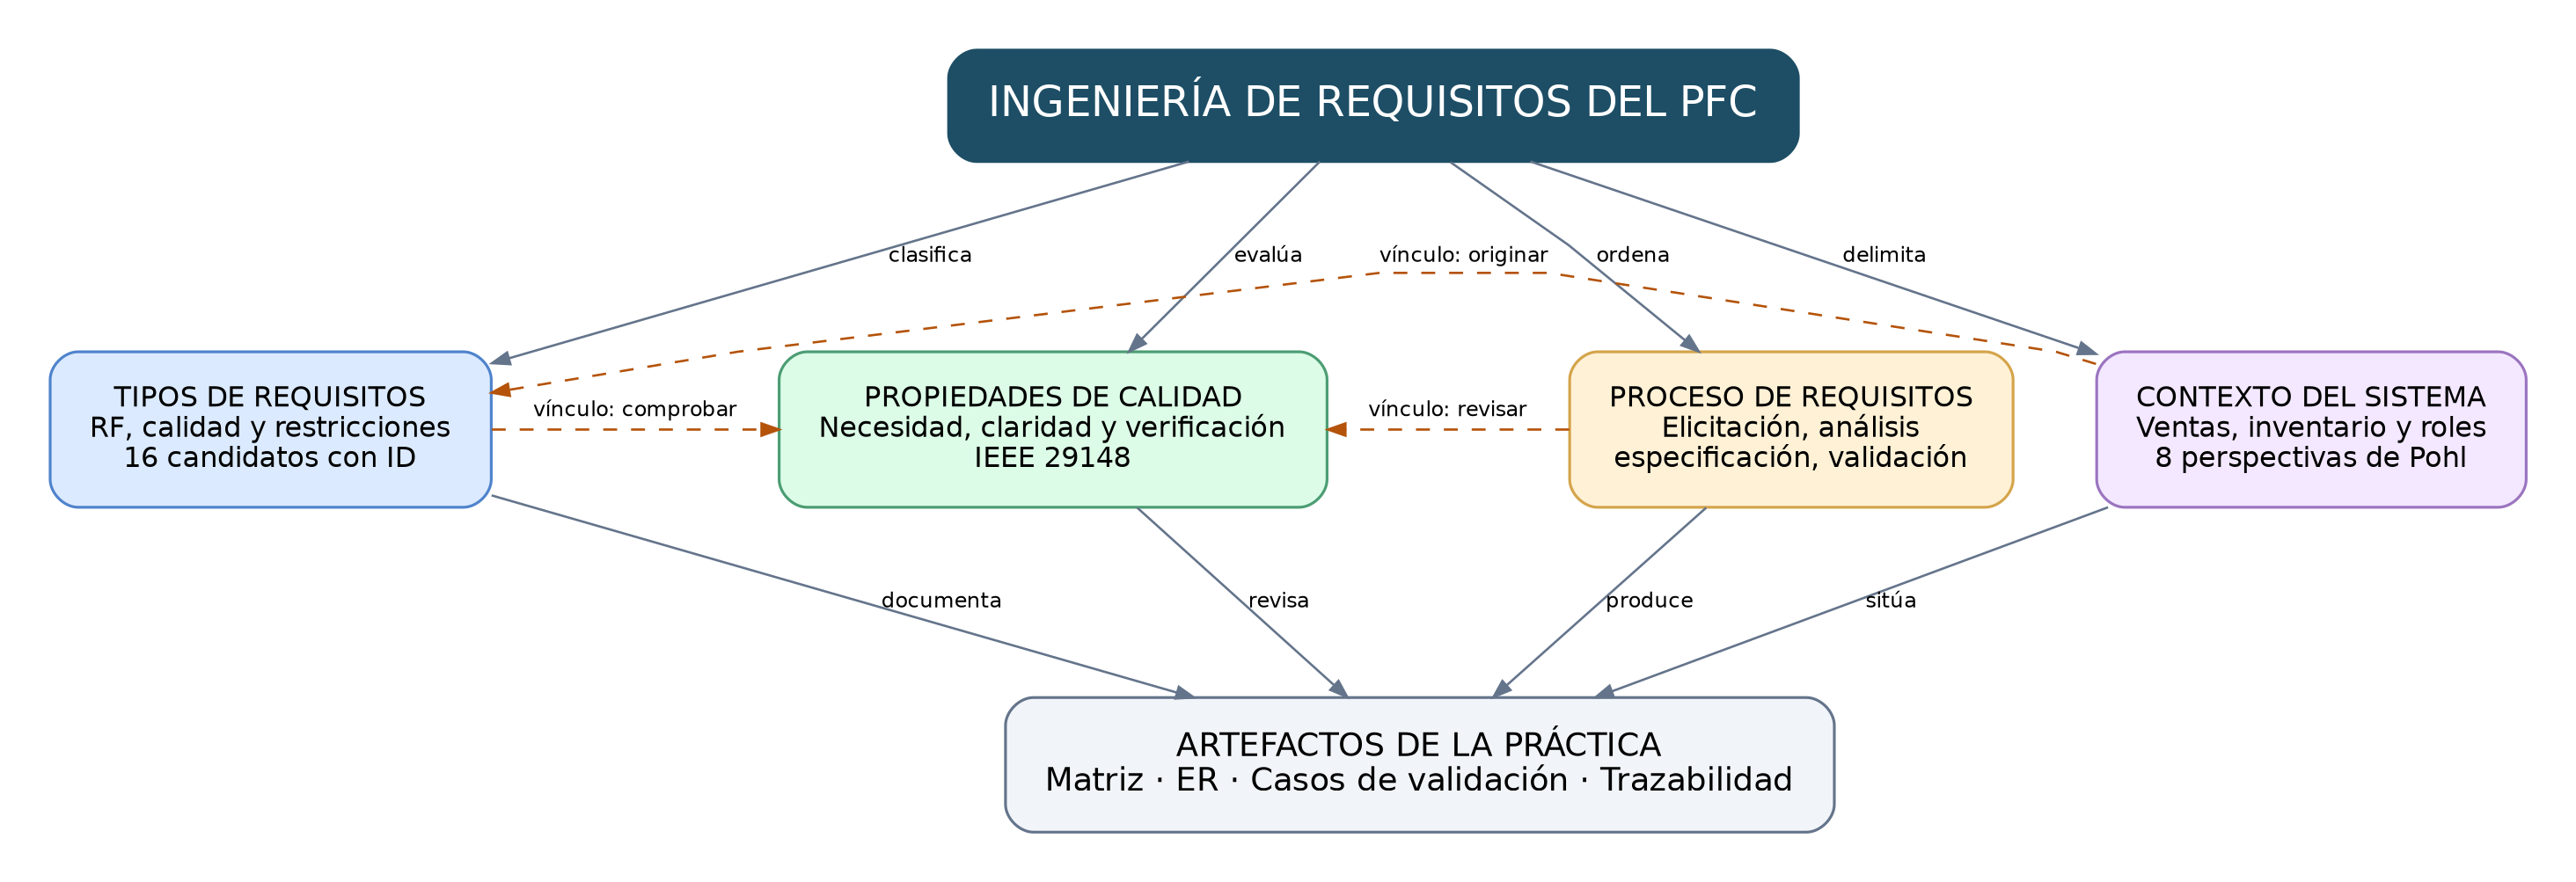
\includegraphics[width=0.92\textwidth]{figuras/mapa_conceptual.png}
\caption{Mapa conceptual integrador de Ingeniería de Requisitos. Las líneas discontinuas representan vínculos cruzados entre temas y todas las actividades se relacionan con artefactos del PFC.}
\label{fig:mapaUnidad}
\end{figure*}
\subsection{Cómo se relaciona con el sistema de ventas}
El problema de caja y de asesoramiento técnico determina el contexto; ese contexto origina los requisitos de búsqueda, venta, inventario y sugerencias. La calidad de los enunciados permite comprobar que no mezclen funciones con restricciones y que incluyan condiciones de aceptación cuando corresponde. El proceso de Ingeniería de Requisitos obliga a confrontar estas propuestas con la documentación disponible y, posteriormente, con los usuarios. El diagrama ER aporta un modelo preliminar de datos, mientras que el mapa conceptual aporta la relación entre las decisiones del proyecto y los temas de la unidad. Ninguno de los dos sustituye la validación de necesidades por la empresa.
